\subsection{Einleitung}

\begin{figure}[H]
	\centering
	\begin{tikzpicture}
		\begin{axis}[
				default,
				xmin=-0.5, xmax=4.5,
				ymin=-0.5, ymax=4.5,
				width=8cm,
				axis lines=middle,
				clip=false,
				xticklabels={},
				yticklabels={}
			]
			\addplot [
				draw=color1,
				pattern=north west lines,
				pattern color=color1,
				opacity=0.5,
				const plot mark right,
				samples=4,
				domain=0.5:3.5]
			{0.2*(x-2)^(3)+0.2*x^(2)+2}\closedcycle;
			\addplot [
				draw=color2,
				fill=color2!30,
				opacity=0.5,
				ybar interval,
				samples=4,
				domain=0.5:3.5]
			{0.2*(x-2)^(3)+0.2*x^(2)+2}\closedcycle;
			\addplot[color3, smooth, thick, domain=0:3.6]{0.2*(x-2)^(3)+0.2*x^(2)+2};

			\draw (0.5, 0.2) -- (0.5, -0.2);
			\draw (2, 0.2) -- (2, -0.2);

			\node[below] at (0.5, -0.2) {\(a\)};
			\node[below] at (3.5, -0.2) {\(b\)};

		\end{axis}
	\end{tikzpicture}
	\qquad
	\begin{tikzpicture}
		\begin{axis}[
				default,
				xmin=-0.5, xmax=4.5,
				ymin=-0.5, ymax=4.5,
				width=8cm,
				axis lines=middle,
				clip=false,
				xticklabels={},
				yticklabels={}
			]
			\addplot [
				draw=color1,
				pattern=north west lines,
				pattern color=color1,
				opacity=0.5,
				const plot mark right,
				samples=7,
				domain=0.5:3.5]
			{0.2*(x-2)^(3)+0.2*x^(2)+2}\closedcycle;
			\addplot [
				draw=color2,
				fill=color2!30,
				opacity=0.5,
				ybar interval,
				samples=7,
				domain=0.5:3.5]
			{0.2*(x-2)^(3)+0.2*x^(2)+2}\closedcycle;
			\addplot[color3, smooth, thick, domain=0:3.6]{0.2*(x-2)^(3)+0.2*x^(2)+2};

			\draw (0.5, 0.2) -- (0.5, -0.2);
			\draw (2, 0.2) -- (2, -0.2);

			\node[below] at (0.5, -0.2) {\(a\)};
			\node[below] at (3.5, -0.2) {\(b\)};

		\end{axis}
	\end{tikzpicture}
	\qquad
	\qquad
	\begin{tikzpicture}
		\draw [color1, pattern=north west lines, pattern color=color1, opacity=0.5] (0, 0) rectangle (0.5, 0.5);
		\node[right] at (0.5, 0.25) {Obersumme};
		\draw [color2, fill=color2, opacity=0.5] (0, -0.5) rectangle (0.5, -1);
		\node[right] at (0.5, -0.75) {Untersumme};
	\end{tikzpicture}
	\qquad

	\caption{Herleitung der Integralfläche über Rechtecke}
\end{figure}

\[
	\Delta x = \frac{b - a}{n}
\]

\begin{align*}
	\text{Obersumme:\quad}  & O = \sum^n_{i=1} f(x_M) \cdot \frac{b-a}{n} \\
	\text{Untersumme:\quad} & U = \sum^n_{i=1} f(x_m) \cdot \frac{b-a}{n}
\end{align*}

\begin{align*}
	\limtoinfty{n} U = A = \limtoinfty{n} O = \limtoinfty{n} \sum_{i=1}^n f(x_M) \cdot \frac{b-a}{n} \\
	 & = \int_a^b f(x) \,\mathrm{d} x \qquad \text{bestimmtes Integral}                              \\
	 & = F(b) - F(a) = {\left[F(x)\right]}_a^b = F(x) |_a^b
\end{align*}

\begin{figure}[H]
	\centering
	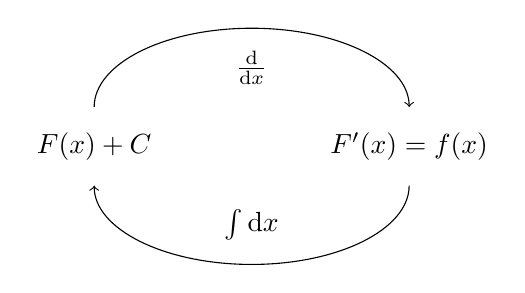
\begin{tikzpicture}
		\node at (0, 1) {\( F(x) + C \)};
		\node at (4, 1) {\( F'(x) = f(x) \)};
		\node at (2, 2) {\( \frac{\mathrm{d}}{\mathrm{d} x} \)};
		\node at (2, 0) {\( \int \mathrm{d} x \)};

		\draw[->] (4,0.5) arc [start angle=0, end angle=-180, x radius=2, y radius=1];
		\draw[->] (0,1.5) arc [start angle=180, end angle=0, x radius=2, y radius=1];
	\end{tikzpicture}
	\caption{Ableitung \& Stammfunktion}
\end{figure}
